\section{Usage}
\subsection{Creating configuration file}
As it was mentioned in \textbf{Introduction} in order to configure a digitizer you must
use configuration file for \blt{WD}. The complete instruction how to create it see in
\blt{WD} documentation. This section is how to do this using the GUI presented in this
package. Here there will be no explanation of what each configure option means, for this,
please, check \blt{WD} documentation.

Firstly, open terminal and change to the directory when you want to place config-file.
Then run the GUI there:
\begin{lstlisting}
> caenccf
\end{lstlisting}
You will see the GUI's starting page (see~Fig.\ref{fig:gui_stpg}).
All configure options have the same names as in the official \blt{WD} documentation so
using is straightforward. However, some things require additional explanation. 
\subsubsection*{Pages}
The GUI consists of four pages (including the starting page). The \codet{Common Settings}
page contains configure options applied to each channel. The \codet{Individual Settings}
page is for the channels' configuration. The \codet{Terminal} settings contains terminal
frame for running \blt{WD} (see below).
\subsubsection*{Path to file}
It is possible to place config-file in a directory that differs from that in which the
GUI was launched. To save config-file wherever you wish use the \codet{Save to} entry

\begin{figure}[H]
    \centering
    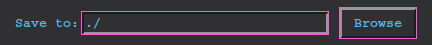
\includegraphics[width=0.4\textwidth]{../pictures/documentation/gui/path.png}
\end{figure}

By default it is the current directory (\codet{./}) but it can be changed either by
changing the entry directly or by using file browser: \codet{Browse} \inlinegraphics{../pictures/documentation/gui/browser.png} button.

\subsubsection*{Baseline and DC offset}
\begin{figure}[H]
    \centering
    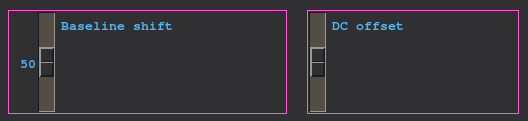
\includegraphics[width=0.4\textwidth]{../pictures/documentation/gui/baseline.png}
\end{figure}
As it is said in \blt{WD} documentation the \codet{BASELINE\tus SHIFT} and
\codet{DC\tus OFFSET} options \emph{are intended to be used one alternatively to the other}.
The GUI reflects this in the following way. If \codet{Use DC offset} \inlinegraphics{../pictures/documentation/gui/check.png} button is OFF then only \codet{Baseline shift} scale matters. Using
\codet{DC offset} scale has no effect. And vice-versa --- if that button is ON only
\codet{DC offset} scale is taken into account.

\subsubsection*{Trigger source option}
There are two choices for trigger: \codet{External} and \codet{Channel}. It seems that
\codet{External} trigger has higher priority for the acquisition. I.e. if you want to
use \codet{Channel trigger} for data acquisition you should choose the corresponding option
in the \codet{Channel trigger} option-menu:
\begin{figure}[H]
    \centering
    
\includegraphics[width=0.4\textwidth]{../pictures/documentation/gui/chan.png}
\end{figure}
\noindent AND disable external trigger in the \codet{External trigger} option-menu:
\begin{figure}[H]
    \centering
    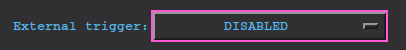
\includegraphics[width=0.4\textwidth]{../pictures/documentation/gui/ext.png}
\end{figure}

\subsubsection*{Saving configuration file} 

Once the configuration is done press \codet{Save} \inlinegraphics{../pictures/documentation/gui/save_btn.png}
button (right lower corner). If succeeded you should see the following popup window
\begin{figure}[H]
    \centering
    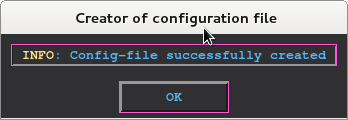
\includegraphics[width=0.4\textwidth]{../pictures/documentation/gui/success.png}
\end{figure} 
\noindent and a file called \codet{config.txt} inside the specified directory.

\subsubsection{Running WaveDump inside GUI}
After successful creation of a config-file it's time to run \blt{WD}.
In the \codet{Terminal} page one will find a frame with running \codet{xterm} inside.
It is intended to eliminate the need for users to use another window to run \blt{WD}.
Go to the \codet{Terminal} page and call \blt{WD} with the path to the config-file you
created before as an argument:
\begin{lstlisting}
> wavedump config.txt
\end{lstlisting}

\Warning{The terminal is running in the directory where the GUI was launched. And if you
chose another directory to save the config-file you must provide the full path to that file.
That is why it is recommended to run the GUI from the directory where you place a config-file.}

In the same page one will find \blt{WD} cheat sheet.  

